%% 该模板修改自《计算机学报》latex 模板
%% 主要是将双栏改成单栏,去掉了部分计算机学报标识;
%% 源文件自:https://www.overleaf.com/latex/templates/latextemplet-cjc-xelatex/ybmmymncrrmw
%% 
%%
%% This is file `CjC_template_tex.tex',
%% is modified by Zhi Wang (zhiwang@ieee.org) based on the template 
%% provided by Chinese Journal of Computers (http://cjc.ict.ac.cn/).
%%
%% This version is capable with Overleaf (XeLaTeX).
%%
%% Update date: 2023/03/10
%% -------------------------------------------------------------------
%% Copyright (C) 2016--2023 
%% -------------------------------------------------------------------
%% This file may be distributed and/or modified under the
%% conditions of the LaTeX Project Public License, either version 1.3c
%% of this license or (at your option) any later version.
%% The latest version of this license is in
%%    https://www.latex-project.org/lppl.txt
%% and version 1.3c or later is part of all distribution`s of LaTeX
%% version 2008 or later.
%% -------------------------------------------------------------------

\documentclass[10.5pt,compsoc,UTF8]{CjC}
\usepackage{CTEX}
\usepackage{graphicx}
\usepackage{footmisc}
\usepackage{subfigure}
\usepackage{url}
\usepackage{multirow}
\usepackage{multicol}
\usepackage[noadjust]{cite}
\usepackage{amsmath,amsthm}
\usepackage{amssymb,amsfonts}
\usepackage{booktabs}
\usepackage{color}
\usepackage{ccaption}
\usepackage{booktabs}
\usepackage{float}
\usepackage{fancyhdr}
\usepackage{caption}
\usepackage{xcolor,stfloats}
\usepackage{comment}
\setcounter{page}{1}
\graphicspath{{figures/}}
\usepackage{cuted}%flushend,
\usepackage{captionhack}
\usepackage{epstopdf}
\usepackage{gbt7714}
\usepackage{listings}
\usepackage{xeCJK}
\usepackage{float}
\usepackage{sourcecodepro}
\usepackage[T1]{fontenc}
\usepackage{hyperref}

\setmainfont{Times Roman}
% \setCJKmainfont{Noto Sans Mono CJK TC}
\setCJKmainfont{標楷體.ttc}
\setmonofont{Cascadia Code}

%===============================%

\headevenname{\mbox{\quad} \hfill  \mbox{\zihao{-5}{ \hfill 2024 Hardware Design  } \hspace {50mm} \mbox{2024 年 11 月}}}%
\headoddname{Group 21 \hfill Final Project Proposal}%

%footnote use of *
\renewcommand{\thefootnote}{\fnsymbol{footnote}}
\setcounter{footnote}{0}
\renewcommand\footnotelayout{\zihao{5-}}

\newtheoremstyle{mystyle}{0pt}{0pt}{\normalfont}{1em}{\bf}{}{1em}{}
\theoremstyle{mystyle}
\renewcommand\figurename{figure~}
\renewcommand{\thesubfigure}{(\alph{subfigure})}
\newcommand{\upcite}[1]{\textsuperscript{\cite{#1}}}
\renewcommand{\labelenumi}{(\arabic{enumi})}
\newcommand{\tabincell}[2]{\begin{tabular}{@{}#1@{}}#2\end{tabular}}
\newcommand{\abc}{\color{white}\vrule width 2pt}
\renewcommand{\bibsection}{}
\makeatletter
\renewcommand{\@biblabel}[1]{[#1]\hfill}
\makeatother
\setlength\parindent{2em}
%\renewcommand{\hth}{\begin{CJK*}{UTF8}{gbsn}}
%\renewcommand{\htss}{\begin{CJK*}{UTF8}{gbsn}}
\renewcommand{\contentsname}{Table of Contents}

\begin{document}

\hyphenpenalty=50000
\makeatletter
\newcommand\mysmall{\@setfontsize\mysmall{7}{9.5}}
\newenvironment{tablehere}
  {\def\@captype{table}}

\let\temp\footnote
\renewcommand \footnote[1]{\temp{\zihao{-5}#1}}

\hypersetup{
  colorlinks=false,
  pdfborder={0 0 0},
}

\thispagestyle{plain}%
\thispagestyle{empty}%
\pagestyle{CjCheadings}

% \begin{table*}[!t]
\vspace {-13mm}


\onecolumn
\zihao{5-}\noindent Group 21 \hfill Final Project Proposal \hfill 2024 年 11 月\\
\noindent\rule[0.25\baselineskip]{\textwidth}{1pt}


\begin{center}
    \vspace {11mm}
    {\zihao{2} \heiti \fangsong Final Project Proposal}
    
    \vskip 5mm
    
    {\zihao{4}\fangsong Group 21: 陳克盈(112062205)、蔡明妡(112062224)}
\end{center}

\lstset{
    % backgroundcolor=\color{red!50!green!50!blue!50},%程式碼塊背景色為淺灰色
    rulesepcolor= \color{gray}, %程式碼塊邊框顏色
    breaklines=true,  %程式碼過長則換行
    numbers=left, %行號在左側顯示
    numberstyle= \small\ttfamily,%行號字型
    keywordstyle= \color{blue},%關鍵字顏色
    commentstyle=\color{gray}, %註釋顏色
    frame=shadowbox%用方框框住程式碼塊
    basicstyle=\ttfamily\footnotesize,
}
 
\definecolor{improvecolor}{rgb}{0,0.6,0} % 深綠色
\definecolor{declinecolor}{rgb}{0.6,0,0} % 深紅色


%%%%%%%%%%%%%%%%%%%%%%%%%%%%%%%%%%%%%%
\zihao{5}
\vskip 10mm
% \begin{multicols}{1}


%%%%%%%%%%%%%%%%%%%%%%%%%%%%%%%%%%%%%%%%%%
%%%%%%%%%%%%%%%%%%%%%%%%%%%%%%%%%%%%%%%%%%

\tableofcontents
\newpage

\section{Introduction}

\subsection{Motivation}
近期比特幣已經突破九萬美元,市值已經突破 9000 年以來所開採的白銀總值,成為全球第八大資產。\
雖然距離全就第一大資產黃金還有很大一段距離,但是從近期走勢,以及加密貨幣 ETF 的興起,\
都顯示加密貨幣已經成為投資者的一大選擇。

近年來高頻交易在金融市場的佔比日益增長,根據研究報導 \footnote{https://www.investopedia.com/terms/h/high-frequency-trading.asp}指出,\
高頻交易在美國股市的交易量佔比穩定在 50\% 以上,而歐洲股市 \footnote{https://www.ecb.europa.eu/press/research-publications/resbull/2020/html/ecb.rb201215~210477c6b0.en.html} \
的佔比則在 24 - 43\% 左右。\

有別於傳統股票市場有著交易所開盤時間的限制,加密貨幣是全球化且全年無休的市場,\
這也使得加密貨幣成為高頻交易的首選,目前高頻交易佔加密貨幣交易所的交易量穩定在 50\% \footnote{https://blog.ueex.com/cryptocurrency-high-frequency-trading-tactics/} 以上,\
其中中國市場更是高達 60 - 80 \% 以上 \footnote{https://www.investopedia.com/news/highfrequency-trading-firms-enter-cryptocurrency-markets/}。

高頻交易除了一般的程式交易之外,也有不少造市商使用 FPGA 能夠實現硬體加速的特性來近一步地降低計算延遲。\
雖然我們無法取得 PCIE 等級的 FPGA 板,但我們仍然能夠使用 FPGA 來模擬高頻交易的環境,這也是為什麼我們選擇這個題目作為我們的 Final Project。

\subsection{Overall Introduction}
在這個專案中,交易將會有兩種模式:
\begin{itemize}
  \item 手動模式:透過鍵盤輸入,模擬交易員手動下單的情況。
  \item 自動模式:FPGA 將會內建幾個自動交易策略,FPGA 讀取交易資料後,\
  便會根據策略發出買賣指令。
\end{itemize}

這兩種模式都將使用 FPGA 作為 IO 與計算的核心,並使用電腦與 FPGA 連接,作為網路封包的傳輸跳板,\
將對應的 API Request 傳送到 Binance 交易所進行交易。

除此之外,FPGA 板也將會透過 VGA 口,將一個輸入匡顯示到螢幕上,讓使用者能夠知道目前所打的指令。

\section{架構}

\subsection{整體架構}

在手動模式下,機器的運作模式主要分成了幾個步驟:
\begin{enumerate}
  \item FPGA 讀取鍵盤輸入,並存入 Buffer 中,並在螢幕上顯示目前的指令
  \item 當 Enter 鍵被按下時,FPGA 會將 Buffer 中的指令透過設計好的 Binary Protocol 傳到 Host 端
  \item Host 端的 Decoder 會將 FPGA 傳來的訊號轉換為對應的 API Request,將其傳送到 Binance 交易所後,\
        再經由 Encoder 將交易結果回傳給 FPGA。
  \item FPGA 收到交易結果後,將相關資訊顯示到螢幕上,並持續監控交易狀況,並根據策略發出額外的交易指令
\end{enumerate}

\begin{figure}[h!]
  \centering
  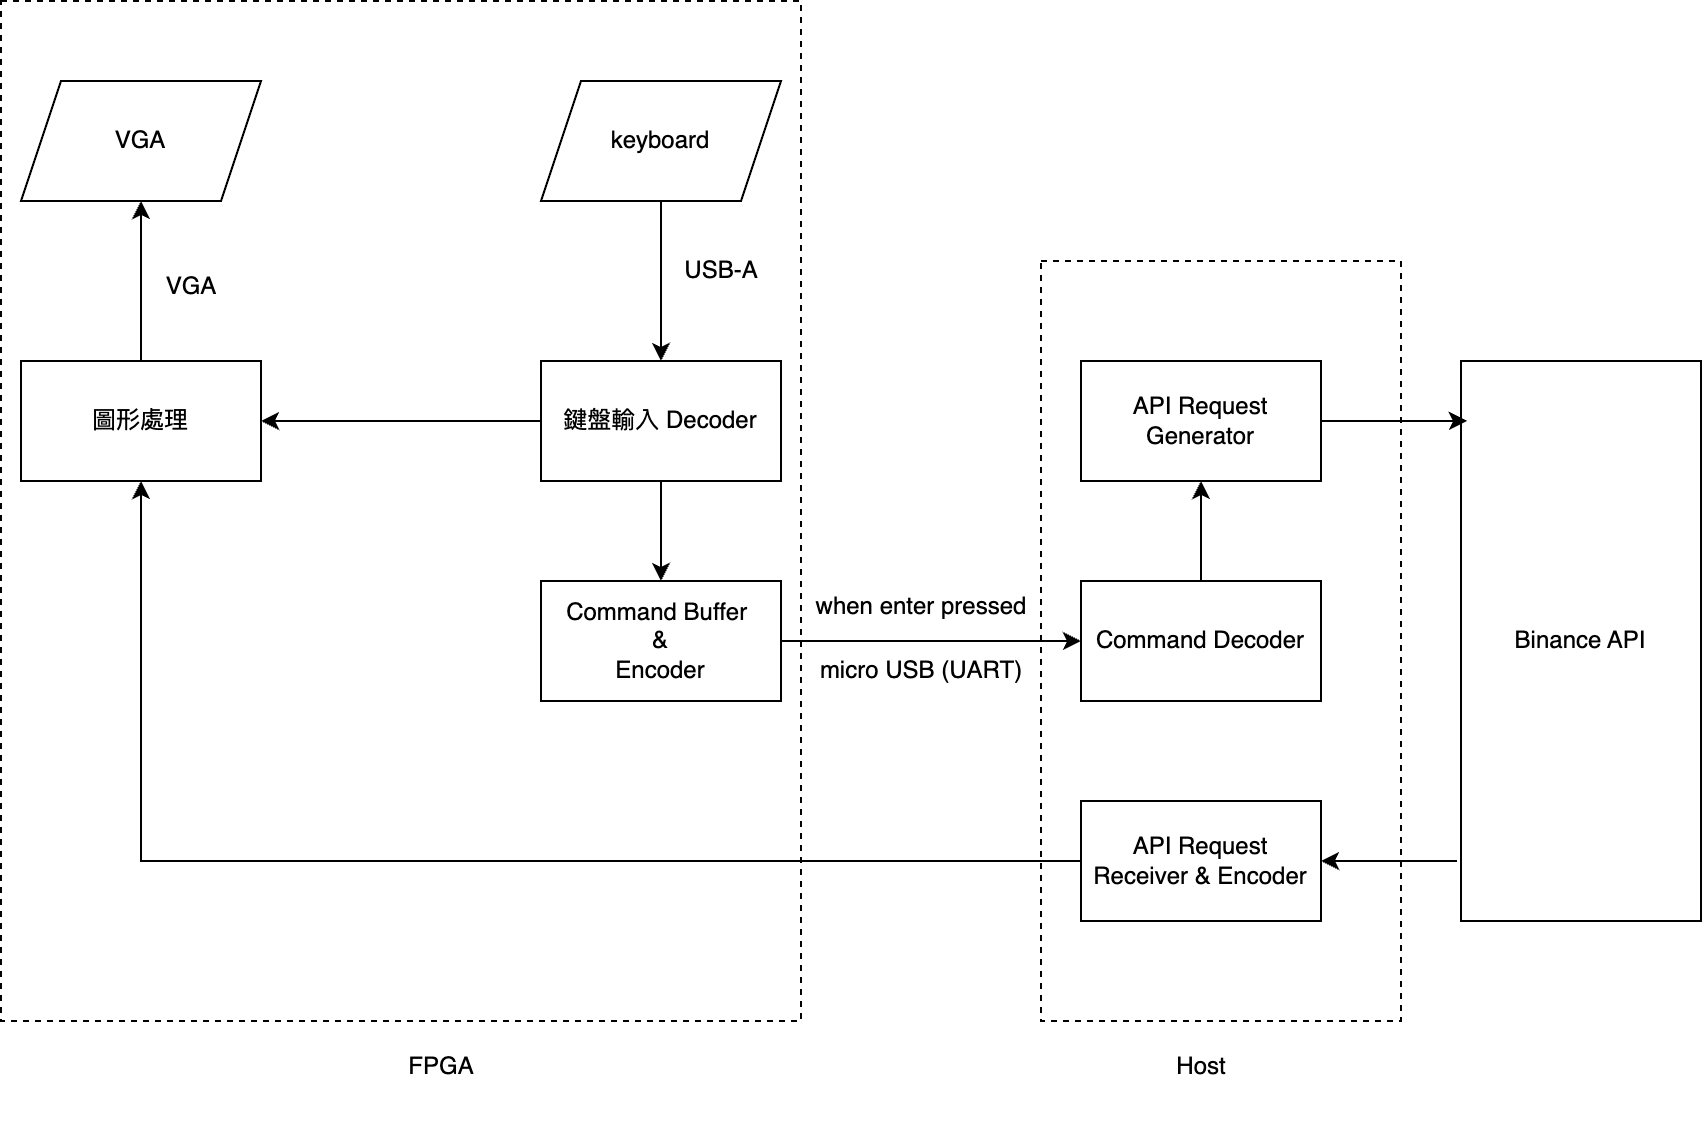
\includegraphics[width=0.8\textwidth]{./img/Final-Project-1.png}
  \caption{手動模式架構}
\end{figure}

在自動模式下,將關閉鍵盤輸入的功能,改由策略模組控制整個交易行為:

\begin{figure}[h!]
  \centering
  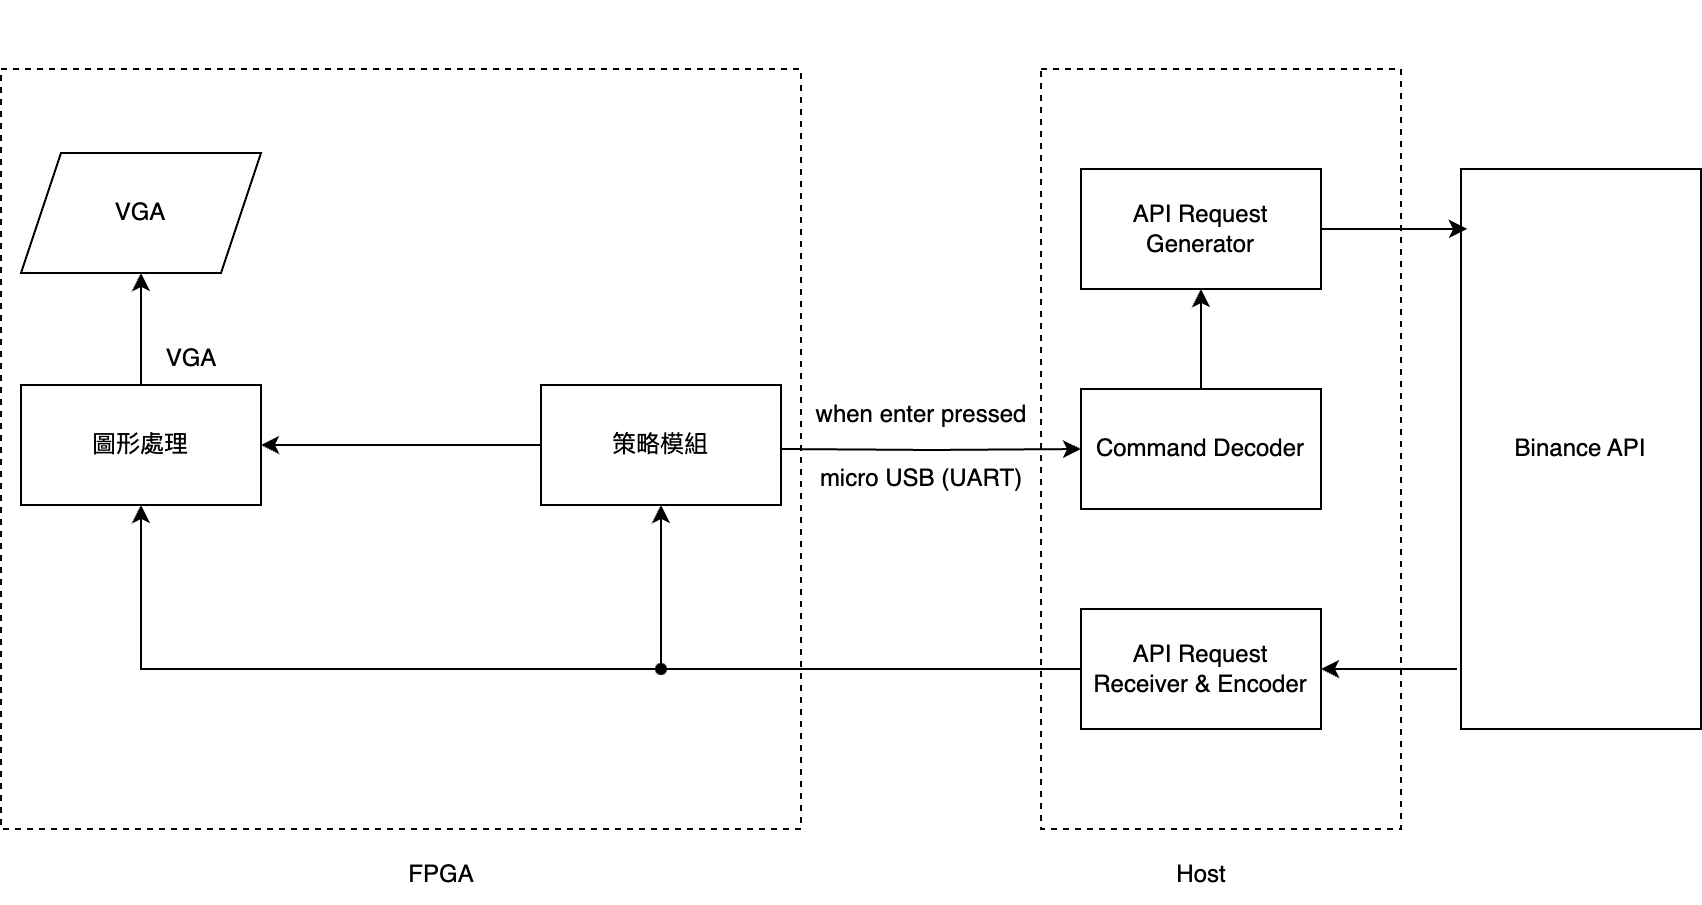
\includegraphics[width=0.8\textwidth]{./img/Final-Project-2.png}
  \caption{手動模式架構}
\end{figure}

\subsection{模組細節}

\subsubsection*{鍵盤輸入 Decoder}

\begin{itemize}
  \item 讀取鍵盤輸入
  \item 支援 Enter, Backspace, Delete, 上下左右等按鍵,讓使用者能夠編輯輸入的內容
  \item 將輸入內容,以 ASCII Code 的方式儲存到 Buffer 中
  \item 實時向圖形處理的 module 發送更新過後的輸入內容
\end{itemize}

\subsubsection*{圖形處理}

將以下資訊轉換為 VGA 訊號顯示到螢幕上:
\begin{itemize}
  \item 鍵盤輸入內容
  \item 交易結果
  \item 帳戶狀態
\end{itemize}

\subsubsection*{Command Buffer \& Encoder}

\begin{itemize}
  \item 儲存鍵盤輸入的內容
  \item 當鍵盤輸入 Enter 時,會將 Buffer 內的指令轉換為在自訂 Protocol 中,\
  該指令所對應到的 Binary Code,並將其透過 UART 的方式傳送到 Host 端
\end{itemize}

\subsubsection*{Command Decoder \& API Request Generator}

\begin{itemize}
  \item 使用 Python 實作
  \item 接收 FPGA 端傳過來的 Binary Code 後,將其轉換為對應的 API Request
  \item 將 API Request 透過 Binance API 送到 Binance 交易所
\end{itemize}

\subsubsection*{API Request Receiver \& Encoder}

\begin{itemize}
  \item 接收 Binance 交易所回傳的交易結果
  \item 將交易結果轉換為 Binary Code,並透過 UART 傳送到 FPGA 端
\end{itemize}

\subsubsection*{策略模組}

\begin{itemize}
  \item 將內建幾種幾單的交易測略,如均線策略、MACD 策略等
  \item 透過 API Request 來取得目前的價格、成交量資訊,並依據策略送出對應的交易指令
\end{itemize}

\section{Budget}

唯一會需要用到錢的只有交易手續費與價差

\section{Timeline}

\begin{itemize}
  \item 11/24 - 11/30:Host 端 API Request
  \item 12/1 - 12/7:鍵盤輸入 \& 圖形處理
  \item 12/8 - 12/14:Command Buffer / Encoder / Decoder
  \item 12/15 - demo:策略模組
\end{itemize}

\end{document}


